% Chapter 2

\chapter{Background information} % Main chapter title
\label{Chapter2} 

%----------------------------------------------------------------------------------------


%----------------------------------------------------------------------------------------

In this chapter, I will firstly make a survey of different types of recommender systems; then I will narrow down the topic to music recommender systems. As music possesses different features comparing to other kind of information such as movie and news, its recommender system also needs to be tailor to bring satisfaction to its listeners.

\section{Overview of recommender systems}
There are currently three main basic approaches to recommendation, namely collaborative recommendation, content-based recommendation, and knowledge-based recommendation \cite{jannach2010recommender}. There is also another type of approach, called hybrid approach, that tries to combine different recommendations together, in order to augment the strengths and limit the drawbacks of each separate technique. The description as well as the advantages and disadvantages of each recommendation techniques will be discussed as follows.

\subsection{Collaborative recommendation}
The main idea of collaborative recommendation approach is to predict potential items that a user would like using past behavior information of other users. Pure collaborative algorithms take only user-item ratings as input and generate predictions suggesting to what degree the user will like a certain item or a list of \textit{n} recommended items as output. 

There are two kind of ratings that can be used, namely implicit ratings and explicit ones. Explicit rating information can be collected by explicitly asking users to rate the item on a specific scale. Different scales are applied to different domains, as the quality of recommendation is different between these scales \cite{cosley2003seeing}. Ratings are then convert internally to numeric values in order for recommender systems to calculate the similarities. Implicit ratings, on the other hand, are knowledge collected based on the interaction between users and the systems. They can be in various forms with distinctive characteristics, such as information about item buying, book reading, music listening, or even user browsing behavior. As implicit ratings are observed behaviors, recommenders have to interpret whether the behaviors have positive or negative impacts toward the users. Even though the interpretation might be incorrect in some cases (e.g., a user might not like all the items that she bought), a massive amount of feedback would exclude these particular cases. In fact, Shafer et al \cite{schafer2006recommender} reported that in some domains, user model using implicit information can outperform the one with explicit ratings.

There are many algorithms developed to exploit the rating matrix; However, in this review, I will just go into detail some main algorithms that have been studied carefully in the past and have been applied widely in the industry. These algorithms include user-based algorithm, item-based algorithm, and an algorithm using matrix factorization/ latent factor models. Some other algorithm, such as probabilistic one, or slope one predictors, are mentioned here because of the scope of the thesis.

\subsubsection{User-based nearest neighbor recommendation}
\textit{User-based nearest neighbor recommendation} is one of the earliest algorithm for this approach. The main idea of the algorithm is to identify users who have similar preferences to a particular user; then for any unknown item \textit{i} of that user, a prediction is given based on the similar of the ratings of other users on item \textit{i}.

\paragraph{Pearson's correlation coefficient}
One common method to calculate the similarity between users is Pearson's correlation coefficient. The general formula for the coefficient \(\rho\) \cite{benesty2009pearson} is:

\begin{displaymath}
\rho_{X,Y} = \frac{cov(X,Y)}{\sigma_X \sigma_Y}
\end{displaymath}

with \(cov(X,Y)\) is the covariance between X and Y, and \(\sigma_X\) and \(\sigma_Y\) represent the standard deviation of X and Y. 

Apply the formula to the case of collaborative filtering: let \( \mathbf{U} = \{ \mathbf{u_1}, \dots, \mathbf{u_n}\} \) denote the set of users, \( \mathbf{U} = \{ \mathbf{p_1}, \dots, \mathbf{p_n} \} \) for the set of items. The 2 sets form a \(n \times m\) matrix of rating \(r_{i,j}\) with \(i \in 1 \dots n, j \in 1 \dots m\), with \(r_{a,p} \) is the rating of user a on item p, and \(\bar{r}_a \) denotes the average rating of user a. The similarity of user a and b \(sim(a, b) \) is defined as follow:

\begin{displaymath}
sim(a,b) = \frac{\sum_{p \in P}(r_{a,p} - \bar{r}_a)(r_{b,p} - \bar{r}_b)}{\sqrt{\sum_{p \in P}(r_{a,p} - \bar{r}_a)^2} \sqrt{\sum{p \in P}(r_{b,p} - \bar{r}_b)^2}}
\end{displaymath}

The Pearson correlation coefficient takes value ranging from -1 to +1, indicating respectively from a strong negative correlation to a strong positive correlation.

\paragraph{Other weighting metrics}
Apart from Pearson's correlation coefficient, other metrics, such as adjusted cosine similarity, Spearman's rank correlation coefficient, or mean squared difference measure are also proposed to calculate user-based similarity. However, empirical study made by Herlocker et al \cite{herlocker1999algorithmic} shows that for user-based recommender system, the Pearson coefficient outperforms other measures.

Still, the "pure" Pearson measure alone is not ideal as there are cases that the measure cannot handle. Consider a real life problem that there are some items that are favored by everyone, Pearson's measure would not consider that an agreement by two users on a controversial item has more weight than an agreement on a universally like item. Herlocker et al \cite{herlocker1999algorithmic} also showed that applying the measure to user who has rated very few items also lead to bad predictions. Therefore, many attempts, such as significance weighting proposed by Herlocker et al \cite{herlocker1999algorithmic}, or case amplification suggested by Breese et al \cite{breese1998empirical} have been made to fill the gap and improve the accuracy. However, the question of whether these weighting schemes are helpful in real-world settings is still opened.

\paragraph{Challenges}
Although user-based approaches have been deployed successfully, they face serious challenges when are applied to large e-commerce sites which possess millions of users and items. Specifically, the cost for scanning a vast number of potential neighbors makes it impossible for the system to predict in real time. Therefore, large scale e-commerce sites often opt for other techniques, one of them is the item-based nearest neighbor approach.

\subsubsection{Item-based nearest neighbor recommendation}
The main idea of this approach is to calculate the similarity between items instead of one between users. The advantage of this approach over user-based approach is that we can preprocess an item similarity matrix that characterize the degree of similarity between items. At run time, a prediction for product p and user u is made by detecting the most relevant items using the item similar matrix and by calculating the weighted sum of u's rating for these items. As the number of relevant item is commonly limited, the computation of the prediction can be done within a short time frame, suitable for such online applications. A similar matrix is, theoretically, also possible with user-based approaches; however, in real time scenarios, the number of overlapping ratings for two random users is relatively small, making it unstable as a few more ratings may significantly affect the similarity between users.

For item-based approaches, the cosine similarity is found to be the standard metric \cite{jannach2010recommender}. The cosine similarity is defined as follows:

\begin{displaymath}
sim(\overrightarrow{a}, \overrightarrow{b}) = \frac{\overrightarrow{a} \cdot \overrightarrow{b}}{|\overrightarrow{a}| * | \overrightarrow{b} |}
\end{displaymath}

where \( \overrightarrow{a} \) is an item vector, \( \cdot \) denotes the dot product, and \(|\overrightarrow{a}| \) is the Euclidian length of the vector, which is defined as the square root of the dot product of the vector with itself. 

One drawback of cosine measure is that it does not take into account the fact that different users have different rating schemes, i.e., some users rate items highly in general, while some others give lower ratings. This drawback is solved using adjusted cosine measure, which subtracts the user average from the rating. Let \( U\) be the set of users that rate both item \(a\) and \(b\). The adjusted cosine measure is as follows:

\begin{displaymath}
sim(a,b) = \frac{\sum_{u \in U}(r_{u,a} - \bar{r}_u)(r_{u,b} - \bar{r}_u)}{\sqrt{\sum_{u \in U}(r_{u,a} - \bar{r}_u)^2} \sqrt{\sum{u \in U}(r_{u,b} - \bar{r}_u)^2}}
\end{displaymath}

with \(\bar{r}_u \) is the average rating for item u.

The prediction function, which is computed in real time, is defined as follows:

\begin{displaymath}
pred(u,p) = \frac{\sum_{i \in ratedItem(u)}{sim(i,p) * r_{u,i}}}{\sum_{i \in ratedItem(a)}{sim(i,p)}}
\end{displaymath}

Compare to user-based recommendation, item-based approach proves to be often more scalable as for most of the case, the number of item falls behind the number of user, thus it requires less time and space to compute the similarity matrix (if necessary). Also, item-based approach is more justifiable by users, for they can easily grasp the explanation of the recommendation, modify the list of neighbors and alter the weights. User-based method, on the other hand, is less able to justify, as recommendations come from other users are hard to explain. However, as item-based approach is based on ratings on similar items, the recommender tends to suggest items that might be already familiar to that user. While this behavior leads to safe recommendations, it does not help users explore other novel items that they might like as well.

In general, nearest neighbor approaches work well for popular items. Nonetheless, there are two important drawbacks with these approaches when deal with unpopular ones:

\begin{itemize}
\item[•] Limited coverage: both approaches define neighbor as having ratings in common. This assumption is limiting, as users with very few common items can still have similar preferences. Moreover, coverage of such approaches can be limited, as only items rated by neighbor are recommended.

\item[•] Sensitive to sparse data: For most system, users only rate a small portions of available items. This results in a cold star problem, when some items have very few or no rating at all, which affects the prediction of these items. Another problem is when there are only few ratings, the weight of each item has a significant impact over the similarity between vectors, reducing the accuracy of the recommender. 
\end{itemize}

To solve these problem, many small tunes for the neighborhood approaches have been made, such as the use of Significance Weighting \cite{bellogin2014neighbor} for the weighting problem or active learning for the Cold Start problem \cite{elahi2014active}. Besides that, other advance algorithms have also been developed to tackle these topics. One of the most popular approaches that has gained attraction recently is the use of matrix factorization, which was exploited to significantly improve the accuracy of the recommender system in the Netflix Prize competition in 2009.

\subsubsection{Matrix factorization/ latent factor model}
Matrix factorization methods is used to derive a set of salient patterns from user-ratings. For example, let "Gone with the wind" and "Me before you" be the set of liked item of user A, and "Romeo and Juliet" and "The fault in our star" be the set of liked item of user B, while nearest neighbor approaches would consider these books separately, matrix factorization could see that both books belong to romantic genre and therefore recommend them to the other user. The factors, however, is not always obvious. In some cases, they can be uninterpretable.

The idea of this method is to factorize the original sparse matrix into a product of matrices. Each decomposed matrix is much denser than the original one. The technique can be used for both similarity matrix and rating matrix. There are many matrix factorization techniques with increasing complexity and accuracy. For the scope of this thesis, I will describe the Singular value decomposition (SVD) model, a basic yet effective decomposition technique. The example is an adaptation from the one from Grigorik \cite{Grigorik2017}. 

Consider the table 2.1:

\begin{table}
\centering
\begin{tabular}{c c c c c}
\hline\hline
& User 1 & User 2 & User 3 & User 4 \\
\hline
Item 1 & 3 & 4 & 3 & 1 \\
Item 2 & 1 & 3 & 2 & 6 \\
Item 3 & 2 & 4 & 1 & 5 \\
Item 4 & 3 & 3 & 5 & 2 \\

\hline\hline \\
\end{tabular}
\caption{Rating for SVD-based recommendation}
\label{table:1}
\end{table}

SVD takes a m-by-n matrix M and decomposes it into three factors: two unitary matrices U and V, which represent the user matrix and the item matrix accordingly, and a nonnegative diagonal matrix \(\Sigma \). The main point of this decomposition is that after receiving the product matrix, we can retain only the most important values in the diagonal matrix to build back the approximation of the original matrix. The decomposition is as follows:

\begin{displaymath}
M = U \Sigma V^T
\end{displaymath}

where \(V^T\) is the transpose matrix of V. 

Applying the decomposition, we obtain \(\Sigma = {12.2215, 4.9282, 2.0638, 0.2977} \) and the two matrices

\hfill \break

%\begin{minipage}[t][5cm][t]{\dimexpr0.5\textwidth-0.5\Colsep\relax}
\begin{minipage}[t]{0.5\textwidth}

\begin{tabular}{c c c c}
\hline\hline \\
U \\
\hline \\
-0.4312 & 0.4932 & -0.5508 & -0.5172 \\
-0.5327 & -0.5305 & 0.4197 & -0.5085 \\
-0.5237 & -0.4052 & -0.4873 & 0.5693 \\
-0.5059 & 0.5578 & 0.5321 & 0.3871 \\
\hline\hline \\
\end{tabular}

\end{minipage}\hfill
%\begin{minipage}[t][5cm][t]{\dimexpr0.5\textwidth-0.5\Colsep\relax}
\begin{minipage}[t]{0.5\textwidth}
\begin{tabular}{c c c c}
\hline\hline \\
V \\
\hline \\
-0.3593 & 0.3677 & -0.2961 & 0.8050 \\
-0.5675 & 0.0880 & -0.6285 & -0.5246 \\
-0.4429 & 0.5686 & 0.6590 & -0.2150 \\
-0.5939 & -0.7306 & 0.2882 & 0.1746 \\
\hline\hline \\
\end{tabular}
\end{minipage}%

In this case, we can eliminate the two dimensions with the lowest values and only keep the two dimensions with value \(\Sigma = {12.2215, 4.9282} \). Figure 2.1 is the projection of the two matrices in a two-dimensional space.

\begin{figure}[h]
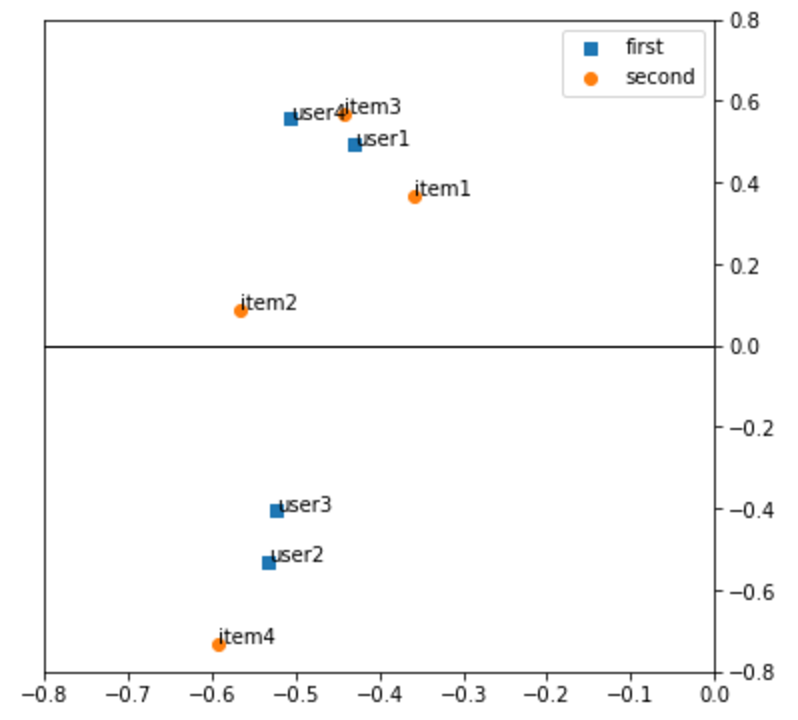
\includegraphics[width=8cm]{SVD}
\centering
\caption{Projection of user and item on a two-dimensional space}

\end{figure}

After the product matrices are constructed, a new user profile can be added by multiply user's rating with the user matrix U and the diagonal matrix \(\Sigma\). Once the user profile is constructed, many strategies can be used for the recommendation of item to that user. One possible approach is to again apply cosine similarity measure to find neighbor user. Another approach is to approximate user rating by exploiting the interaction between user and item in the latent factor space \cite{koren2009matrix}.

\subsection{Content-based recommendation}
Although collaborative filtering approaches work well, they still have some limitations. Apart from the cold star problem and the popularity bias, collaborative approaches require lots of user rating for the system to be stable. Besides, these approaches cannot take advantage of the semantic content of the item. For example, it would be obvious to recommend "Gone with the wind" to a user, if we know that (a) this book belongs to romantic catalog and (b) the user has an affair for romantic novel. Therefore, as data are becoming more abundant, new approaches, commonly called content-based recommendation, have been studied to exploit these data for the recommendation process.

The basic idea of content-based approaches is to classify similar items using a list of features of each item. For example, a book recommender could use the metadata of the book, such as the author's name and the book's genre as a reference for similarity; or it could calculate the similarity of two books based on the overlap of keywords, using the Dice coefficient \cite{salton1988syntactic} as follows:

\begin{displaymath}
sim(b_i, b_j) = \frac{2 * |keywords(b_i) \bigcap keywords(b_j)| }{|keywords(b_i)| + |keywords(b_j)|}
\end{displaymath}

with \( |keywords(b_i)| \) is the number of keyword in book \(b_i\).

However, metadata also need the clarification of expert. The standard approach in content-based recommendation is, not to maintain a list of metadata, but to seek for the similarity in the content of the item itself. In the case of book recommender, one common approach is to transform the content of a book into a vector in a multidimensional Euclidian space using \textit{term frequency-inverse document frequency (TF-IDF)} technique. For the scope of this thesis, the detail of the technique is not described here.

Music recommender systems, however, take a different approach compare to other text recommender sytems, as the differences in characteristics between the two items. Metadata of a music track can include general tags generated by expert such as genre, artist, album, etc..., as well as other social tags by users; and the content of a track is the acoustic features that are analyzed from the signal of that track, of which the most representative ones are timbre and rhythm \cite{cano2005industrial}.

Basically, a content-based recommender has three basic components \cite{ricci2011introduction} 

\begin{itemize}
\item[•] Content analyzer: the mission of this component is to extract relevant information from the  content of the item. In this phase, feature extraction techniques are used to exploit information and transform them to the representation that the recommender needs. The representation is the input to the \textit{profile learner} and \textit{filtering component} parts.

\item[•] Profile learner: in this phase, the module tries to construct user profiles using the representation of the item. Often, this phase is achieved through the use of various kind of machine learning techniques \cite{mitchell1997machine}, depending on the nature of input data. User profiles are then passed into filtering component for generating list of recommendations.

\item[•] Filtering component: This phase generates a list of recommendation for the users by comparing the similarity between the representation of user profiles and that of items to be recommended. After recommendation is suggested, the system might get feedback of the users for the profile learner phase to improve the user profiles.

\end{itemize}

A survey of the techniques used in content-based recommender will be discussed later. For the moment, some music features as well as the techniques that are used to extract them will be described. The profile learner and filtering component parts will not be detailed here, as they are beyond the scope of the thesis. However, the specific algorithms used for these part will be described later in chapter 3. 

\subsubsection{Feature extraction}
Music, in its original form, is a record of analog audio signal (i.e, electrical voltage) \cite{hodgson2010understanding}. To store music digitally, a analog-to-digital conversion is needed. The process has two phases: sampling and quantization \cite{jurafskyspeech}. In the sampling part, a signal is sampled by evaluating its amplitude at a particular time, with the number of samples taken per second is called the sampling rate. The amplitude measurements are then mapped as 8 or 16-bit integers, whose process is called quantization. 

Because digital music is represented as a series of integers, the raw information they contain is trivial for human at the perceptual level. Therefore, the first step of a music recommender is to extract useful features from the raw representation. In music domain, different taxonomies have been created to capture audio features in certain perspectives. Weihs et al. \cite{weihs2007classification} divided audio features into four subcategories, including short term features, long term features, semantic features, and compositional features. Another taxonomy was proposed by Scaringella \cite{scaringella2006automatic}, which separates audio into three different components: timbral to denote features related to spectral content (i.e. shape) of the signal; temporal features such as loudness, tempo, onset rate; and tonal component such as harmonic, pitch, key, scale, and chords distribution. 

Fu et al. \cite{fu2011survey} developed another taxonomy under human understanding of music perspective. According to the hierarchy, there are two level of audio features: low-level and mid-level features. Low-level features are features that can be obtained directly from the audio with proper signal processing techniques like Fourier transform, spectral analysis, autoregressive modeling, etc. Timbral and temporal are two main classes in low-level features. Low-level features have been exploited massively in music classification, due to the simple procedure to obtain and their good performance. However, they are not closely related to the nature of music that human perceive. Mid-level features, on the other hand, delimitate music using rhythm, pitch, and harmony, concepts that are more familiar to normal listeners. 

\paragraph{Low-level features}

Timbral is perhaps the most exploited characteristic in the set of low-level features. It is described as the quality of sound, with different timbres belong to different types of sound sources, e.g. different instruments. Table \ref{table:2} lists some major timbre features. Despite of the large variety in number of features, the timbre extraction phase of all these features are closely related to each other and follow some standard procedures. As this thesis does not deal with low level signal processing, the detail of these procedures is not described here. 

\begin{table}[h!]
\centering
\begin{tabular}{| c | c | c |}
\hline
Class & Feature Type & Used in \\
\hline

\multirow{5}{*}{Timbre} & Zero Crossing Rate & \cite{tzanetakis2002musical}, \cite{li2003comparative}, \cite{bergstra2006aggregate} \\
& Spectral Centroid & \cite{tzanetakis2002musical}, \cite{li2003comparative}, \cite{bergstra2006aggregate}, \cite{morchen2006modeling} \\
& Mel-frequency Cepstrum Coefficient & \cite{tzanetakis2002musical}, \cite{bergstra2006aggregate}, \cite{mandel2006song} \\
& Fourier Cepstrum Coefficient & \cite{bergstra2006aggregate}, \cite{lin2005audio} \\
& Stereo Panning Spectrum Features & \cite{tzanetakis2007stereo}, \cite{tzanetakis2010stereo}\\

\hline

\multirow{3}{*}{Temporal} & Statistical Moments & \cite{tzanetakis2002musical}, \cite{li2003comparative} \\
& Amplitude Modulation & \cite{pampalk2002content}, \cite{pampalk2005improvements} \\
& Auto-Regressive Modeling & \cite{shawe2005investigation}, \cite{meng2007temporal} \\

\hline

\end{tabular}
\caption{Low-level audio features}
\label{table:2}
\end{table}


Timbral features have been successfully used in the past for genre classification. However, it still has several disadvantages. One critical problem is that with the technological advance in the recording process  (e.g., tape editing, equalization, and compression), the final signals of the post production stage of the same instrument in two different tracks would be different. As timbral features techniques rely heavily on raw signal, they are heavily affected by the recording process, of which phenomenal called album effect \cite{whitman2001artist}.

Temporal features are another low-level features that are used to capture the temporal evolution of the signal. The difference between the two features is that, while each timbral is extracted in a local window of raw signal with 10- 100 ms duration, temporal extraction is performed on a series of timbre features in larger frames, allowing for the derivation of a richer set of features, such as fluctuation pattern \cite{pampalk2002content}, rhythmic pattern \cite{lidy2007improving}, rhythmic coefficient \cite{west2009novel}, etc. Morchen \cite{morchen2006modeling} has generated a set of operation that can be employed on top of timbre to produce new features at a coarser scale. Many of these features belong to the amplitude modulation family, as they are generated by analyzing the modulation of the amplitude spectrum. 

\paragraph{Mid-level features}
Low-level features were dominantly applied for genre classification; however, they do not capture the intrinsic properties of music that humans perceive. Mid-level features, such as rhythm, pitch, or harmony, are more familiar to human. Therefore, they play an important role in some specific domains, such as query by singing \cite{jang2008general} or detect cover versions of popular songs with similar melodies \cite{tsai2005query}

Rhythm is the most widely used mid-level feature in audio-based music classification. It describes the recurrence of tension and release in music. From rhythm, "danceability" of a track can be derived by . Rhythm can also be used for mood classification \cite{feng2003music} \cite{yang2004disambiguating}, since sad songs usually have a slow rhythm, while exciting songs usually possess a fast rhythm. 

Pitch is another important mid-level feature. It is defined as the most fundamental frequency of the sound. Often, a pitch histogram is constructed and is combined with low-level feature for genre and mood classification \cite{tzanetakis2002musical} \cite{li2003detecting}. Pitch can also used to develop pitch class profile and harmonic pitch class profile, which in turn are useful for detecting similar melodies and transcription \cite{marolt2006mid} \cite{poliner2007melody}. 

Harmony is a succession of musical chords, which are three or more notes, typically sounded simultaneously. The chord is detected by compare pitch histogram with chord template to identify the possible chords. Chord features are often used as a complimentary to pitch features in detecting melody similarity and cover song \cite{ellis2007identifyingcover} \cite{bello2007audio}

To summarize, low-level audio features such as timbre are sufficient for genre classification but fail to achieve good result in song similarity detection. Mid-level features, on the other hand, are successful in detecting similar song using pitch and harmonic features. Rhythm features have also been exploited for mood classification. Research in using acoustic contents for recommendation problems will be describe later in the overview of music recommender systems part. 

\subsection{Hybrid recommendation}
Hybrid recommendation is a method that combine several kind of recommenders together. The motivation for hybrid recommender is to try to take advantage of the strength of different algorithms with fewer drawbacks than any individual one. Burke's well-known taxinomy \cite{burke2002hybrid} differentiate between seven kind of hybridization strategies; However, the seven approaches can be abstracted into three base design: monolithic, parallelized, and pipelined hybrids \cite{jannach2010recommender}. Monolithic design incorporates several recommendation strategies into one algorithm, while parallelized and pipelined designs require at least two separate recommenders. The outlines of the three designs are depicted in Figure \ref{fig:monolithic}, \ref{fig:parallelized} and \ref{fig:pipelined}

\begin{figure}[h]
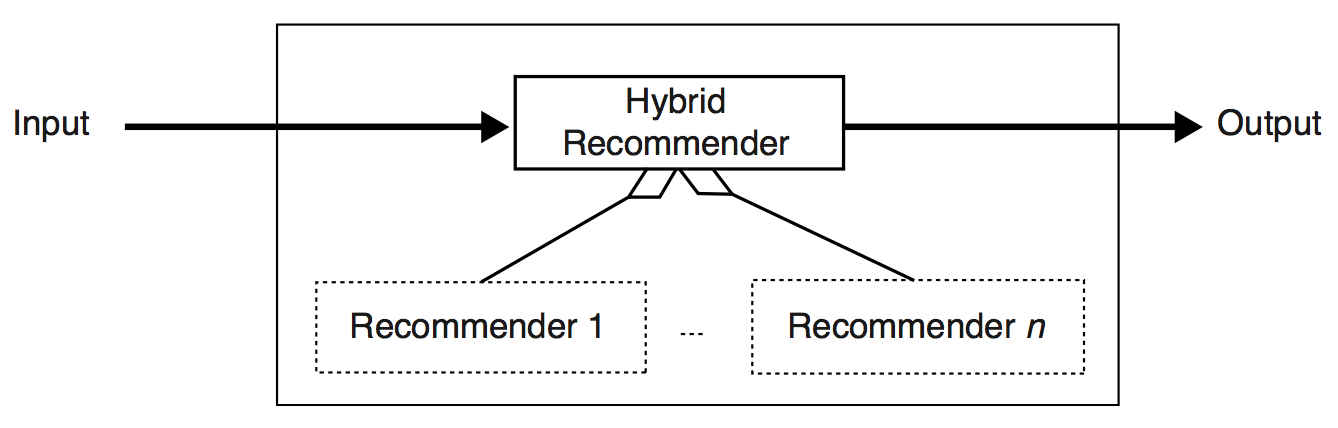
\includegraphics[width=8cm]{monolithic}
\centering
\caption{Monolithic hybridization design}
\label{fig:monolithic}

\end{figure}

\begin{figure}[h]
\includegraphics[width=8cm]{Parallelized}
\centering
\caption{Parallelized hybridization design}
\label{fig:parallelized}
\end{figure}

\begin{figure}[h]
\includegraphics[width=8cm]{Pipelined}
\centering
\caption{Pipelined hybridization design}
\label{fig:pipelined}
\end{figure}

\subsubsection{Monolithic hybridization design}

Monolithic design consist of a single recommender that combines different type of input data and and uses a build-in algorithm to exploit these data for the recommendation process. Feature combination and feature augmentation strategies from Burke's taxonomy \cite{burke2002hybrid} can be assigned to this category. 

A feature combination hybrid is a monolithic recommender that simply combine information from a varied source of input data. For instance, Basu et al. \cite{basu1998recommendation} proposed a hybrid recommender that combines collaborative features, such as users' likes and dislikes of each movie, with genre features of the movie. Therefore, instead of identifying just a group of users who watch the same movies, the recommender determines a group of users who watch same movies of the same genre, such as comedy, drama, or action.

A feature augmentation hybrid is also a monolithic design that combines different source of features. In contrast with feature combination, feature augmentation does not simply combine features, but also apply some transformations so that some features are strengthened as compared to other features. Content-boost collaborative filtering \cite{melville2002content} is an example of this hybrid. The algorithm creates a concept of pseudo-user-ratings, as well as uses different weighting scheme between collaborative features and content features. 

\subsubsection{Parallelized hybridization design}
Parallelized hybridization designs gather result of several recommenders and aggregate their outputs using a hybridization machanism. Mixed, weighted, and switching are three main strategies that are used in the parallel design. 

A mixed hybrid design combines the results of several recommenders at the level of user interface. The top-scoring items are then presented to users in order. However, as items from different recommenders are mixed together, some conflicts might happen. For example, Zanker et al. \cite{zanker2007development} built a mixed system to propose bundles of different product in the tourism domain. One bundle, for example, contains two recommenders, one for accommodations and the other for sport and leisure activities. As the two recommenders are separated, there would be a case when the top-score accommodations are far away from the suggested sport place. Therefore, a Constraint Satisfaction Problem solver is often employed in the design to resolve these kind of conflicts.

A weighted hybrid design also combines the results of different recommenders, then compute the weighted sums of their scores. The weight can be estimate by using an empirical bootstrapping approach \cite{zanker2009case} or a dynamic weighting scheme \cite{claypool1999combing}. 

Switching hybrid strategy assigns which recommender to use under certain situations. For example, to overcome the cold start problem, the system can use the results of content-base recommender until enough user rating are available. When the recommender see a sufficient number of user rating, it starts to use results generated from collaborative filtering recommender. One practical example of this hybrid design is the NewsDude system \cite{billsus2000user} to recommend news articles. First, a content-based nearest neighbor recommender is used. If there is no related articles found, a user collaborative filtering recommender is used to propose cross-genre alternative.

\subsubsection{Pipelined hybridization design}
Pipelined hybrids is a design that the output of a recommender is used as the input of another one with the exception of the final one, whose results are shown to users. Cascade hybrids and meta-level hybrids are two types of this principles. 

In cascade hybrid design, the succeeding recommender can only receive the output of its predecessor. In other words, except the first recommender that process the whole set of items, all other remaining recommenders can only alter the score or exclude the items that endure from their preceders without the ability to add new one. As each recommender have the property of reducing the size of the recommending set, cascade strategies might meet a problem of not proposing enough recommending items. The problem can be solved by combining cascade hybrids with a switching strategy, as applied by Zanker et al. \cite{zanker2009case} to build a cigar recommender system. 

A meta-level hybrid is one that, in the training phase, use a recommender to transform raw data to a model that is then fed into the actual recommender. In the testing phase, however, the contributing recommender is eliminated from the system. That is to say, the raw data in the testing phase is evaluated directly by the actual recommender. This hybrid design is hard to apply, as the contributing recommender has to generate a model that is useful for the actual recommender, and not all recommendation logics can do so.

\subsection{Other kind of recommendation}
So far, collaborative filtering, content-based filtering, and hybrid approaches have been introduced. There are many other kinds of recommendation system, such as knowledge-based recommendation, critique-based recommendation that are used in some specific domains. In the music domain, there are also context-aware recommender system, where the recommenders try to incorporate contextual information, such as time and current activities, into the recommendation process. I will not discuss in deep these methods here, as it goes beyond the scope of the thesis. However, information of recommenders that use contextual information will also be included in the overview of music recommender systems part.

In the next section, recommender systems that are build in music domain will be discussed. Specifically, the kind of information as well as the methods used in content-based and context-based recommendation will be presented. Also, some hybrid designs that combine content, context, and user-rating information will also be introduced. 

\section{Overview of music recommender systems}
Music, differs from other content domains such as books or movies, has its own unique characteristics regarding consumption. For example, the consumption time of books and movies are quite lengthy, ranging on the average of few hours (for movies) to several days (for books); songs, on the other hand, takes a much shorter time for listener to consume, only a few minutes. Consequently, this lead to the ephemeral and disposable nature of music. Another example is the number of repetition: a single song can be consumed repeatedly (even multiple times in a row), while books are movies are consumed a few times at most. This implies that the user might appreciate recommendations of items that they already heard in the past.

In the past, many approaches, based on the observation of the nature of music and listener's behaviors, had been tried to build an efficient music recommender system. Till now, there are three main approaches to such system \cite{ricci2011introduction}, which will be described in the following sections. 

\subsection{Content-Based Music Recommendation}

Content-based recommendation exploits information describing music as material for recommender systems. There are two main approaches for content-based system: one uses metadata, such as annotations or social tags, while the other analyses audio content using machine learning techniques.

\subsubsection{Metadata content}
Metadata comes in several forms. One is the manual annotations constructed by music experts or voluntary community. This kind of annotation often obeys a strict structured taxonomy build by expects. Another form of annotations is social tags, which is built by asking casual users to provide unstructured text annotations for the item. The last kind of annotations is information collected on web pages, blogs and RSS feeds related to music items.

\paragraph{Annotation} 
Manual annotation contain information such as musical genre, record label, year, knowledge about tracks and artists, and albums. Some musical properties, particularly tempo, mood, and instrumentation can also be added. Many online database have been built using editorial metadata, following by many recommender systems trying to exploit them. 

Bogdanov et al. \cite{bogdanov2012taking} build an artist recommender using exclusively metadata from \textit{Discogs}, a free and community-built database containing information about artists, records labels, and their releases. For each artist in the database, a tag weight vector is created using genre, style, label, country, and year information of the releases related to the artist. The role of the artist in each release (e.g. main artist, track artist, or extra artist) and the relations between artist, such as aliases and membership relations, are also taken into account. A sparse tag matrix is then formed from the artist vectors, and latent semantic analysis \cite{deerwester1990indexing} is applied to reduce the dimension of the matrix. Afterwards, the authors use Pearson correlation distance \cite{gibbons2011nonparametric} to measure the similarity between artists.

Apart from community-built database, some other database are developed by experts for commercial use. \textit{Pandora}, for example, is a personalized radio that built its recommender using annotations done by experts \cite{jones2007user}. \textit{AllMusic} is another example that also provides mood annotations besides general editorial metadata. However, not much research has been done using these database, as they are proprietary, and there is no public data sets of this kind are available for researcher. Constructing such a data set would be costly, and they are difficult to scale to large collections.

\paragraph{Social tags}
Social tags are tags provided by user using the services. Tags are personalized, arbitrary, and do not follow any particular structure, ranging from genre like "blue" or "jazz" to event-related attributes (e.g. "live") and assertion (e.g. "my favorite song"). They also vary in scope, from broad one such as "classical" to niche terminology like "Malcolm Arnold" or "renaissance". Social tags, therefore, need to be preprocess for the data to be useful. A popular method, which is used by \textit{Last.fm}, a social music website, for structuring social tags is to transform them into a folksonomy \cite{sordo2008quest}. The tag weight vectors technique is then applied to compute the similarity \cite{green2009generating}, with the enhancement by using latent semantic analysis techniques to overcome vector sparsity problem \cite{levy2008learning}

\paragraph{Annotations by web crawling}
Apart from tags made by experts and social tags, some recommender systems are built using information crawled from web pages. These recommenders often apply artist similarity metric, generated by using text mining techniques \cite{schedl2011exploring}, as the main principle for the recommendation. Green et al. \cite{green2009generating} compute artist-to-artist similarity using keyword extracted from \textit{Wikipedia} entries and social tags from \textit{Last.fm}. Similarly, McFee and Lanckriet \cite{mcfee2011learning} predict artist similarity based on social tags and keyword extracted from artist biographies on \textit{Last.fm}. A deviant approach is the one made by Lim et al., as they compute song-level similarity through bag-of-words representations of lyrics found on \textit{musiXmatch.com} \cite{lim2013robust}

\subsubsection{Audio content}
Audio content analysis is promoted by MIR researchers as an alternative to metadata and collaborative filtering method \cite{barrington2009smarter}. Content analysis is expected to solve "long tail" problem, where unpopular music items are not suggested because the lack of available user ratings, tags, and other types of metadata \cite{celma2009music}. Music content is separated into two broad categories: acoustic features taken directly from the audio, and semantic annotations derived from acoustic features using machine learning techniques. 

\paragraph{Acoustic features}
Acoustic features are properties 	of a sound that can be recorded and analyzed using signal processing techniques. As mentioned in the content-based recommendation part, there are three main features that are often used by recommender system: timbral features, temporal and time-domain features, and tonal features.

Timbral similarity method converts timbre information to a standard representation and applies a number of methods to approximate the likelihood between two songs \cite{aucouturier2005way} \cite{logan2001music}. For example, Logan \cite{logan2004music} builds a recommender that compares Mel-frequency cepstrum coefficient (MFCC) based distance of user's music set with target play list. The approach, however, is insufficient as evaluation shows a nominal number of customer satisfaction \cite{bogdanov2013semantic}. 

Pampalk et al. \cite{pampalk2005improvements} \cite{pampalk2005dynamic} study an algorithm that use, in addition to spectral similarity, loudness fluctuations and two derived descriptors from sound wave to improve the accuracy of music similarity and genre classification of a song. The algorithm is used to recommend user playlists, in which songs that are similar to the ones that are skipped by user are eliminate, and only tracks that are similar to the ones that the user wholly listens to remains.

Celma and Herrera \cite{celma2008new} take another approach, calculating Euclidean distance using timbre, dynamics, tempo, meter, tonal strength, key, and mode information. This method is compared to an item-based collaborative filtering and a hybrid method on a large scale evaluation. The result shows that all three algorithms work fine recommending familiar items. For unfamiliar items, collaborative filtering reveals a poor discovery ratio, while pure content-based method sometimes goes off direction, as the recommender confuse between similar sounds, such as between the sound of classical guitar and the one of harpsichord). The hybrid method performs the best, as it limit the number of possible tracks whose artists are related with the original artist, therefore reducing mistakes performing by pure content-based method.

\paragraph{Semantic annotation}
Pure acoustic signal, unfortunately, cannot directly capture semantic meaning of a track. As a result, mere acoustic feature recommenders do a poor job in song suggestion, as an "energetic" song can be recommended next to a "nostalgic" track because of the similarity of the instrument. A sudden change in genre might frustrate customer, as one would not expect a mourning song in a middle of a party. Therefore, many approaches have been made in order to bridge this semantic gap by using machine learning techniques to predict annotations from audio content.

However, extracting genre or mood information from acoustic content is perplexing, as mapping between human annotation and acoustic cannot be clearly defined \cite{aucouturier2009sounds}. To solve this,  Barrington et al. \cite{barrington2009smarter} propose a method to measure semantic similarity: they train Gaussian mixture models of MFCCs for semantic concepts such as genres, moods and instruments. Therefore, for a song, a distribution of tags is generated, which is then compared to another in order to estimate similarity. 

\subsection{Contextual Music Recommendation}
The vast majority of existing recommender system approaches focus on information about users and items but not context information, such as time and place of the event. Only until recently, the topic of context-awareness starts to gain attraction in recommender system research \cite{adomavicius2011context}. Context, in the fields that are directly related to recommender system, is defined as "information describing where you are, whom you are with, and what resources are nearby" \cite{schilit1994context}. Therefore, context in the domain of music can be derived as a collection of factors that affects user's appreciation of music, such as time, mood, and current activities.

Contextual information can be classified using various kind of classifications. Adomavicius et al. \cite{adomavicius2011context} suggest categorizing context into three distinct classes: fully observable, partially observable, and unobservable context. Dey and Abowd \cite{abowd1999towards}, in attempt to construct another classification, propose to classify context into primary context, which is four most important factors that describe user situation: location, identity, activity, and time; and secondary context, which is data derived from primary information. Applying the classification of Dey and Abowd, M. Schedl et al \cite{schedl2015music} divide context information into two generic classes: environment-related context and user-related context. Environment-related context refers to information that can be obtained by user's computer or mobile phone, such as location, time, weather, etc., while user-related context indicates information that can be derived from the environment-related one, such as user's activity, emotion state, and social environment. 

\subsubsection{Environment-Related Context}
Surrounding environment has been proven to have an influence on user's preference of music. Adrian C. North and David J. Hargreaves \cite{north1996situational} find a correlation between musical descriptors, such as arousal, sensuality, spirituality, and listening situation, such as activity, spirituality, and social constraint. Pettijohn et al. \cite{pettijohn2010music} find that different seasons, such as winter and summer, also affect musical preferences. 

Many attempts have been made to build recommender using environment-related information. Reddy and Mascia \cite{reddy2006lifetrak} used space information capturing using GPS coordinates, internal time data, kinetic information derived from difference in GPS signals, and even meteorological info to build a recommender for a mobile music player called Lifetrak. Songs have to be tagged manually by users using system predefined tagging system, and are played in appropriate situation based on users' preferences. For example, the app may play rock music when a user is in a gym, and classical music when the user tries to study in a cafeteria. 

Ankolekar and Sandholm from HP labs \cite{ankolekar2011foxtrot} propose a mobile audio application, Foxtrot, that exploits crowd-sourced geo-tagged audio information to provide a stream of location-aware audio content to the users. The recommender, however, generated poor user experiences, as an environment generates different meaning to different people, leading to diverse music preferences. Indeed, a research made by Okada et al. \cite{okada2013contextplayer} shows that not only the algorithm, but also the architectural design and usability of the application that matter, as user feedback suggests the need for explanations of the recommendations and more control over the playlist. 

\subsubsection{User-Related Context}
One's music preference is not only affected by geological and activity component, but also by factors such as emotions and social background. Sch{\"a}fer and Sedlmeier \cite{schafer2009functions} discovered that one's music preference is also linked with one's sociocultural and physiological functions. In other words, people use music preference as a mean to express their identities and personal values. User-related context can be divided into the following groups:

\begin{itemize}
\item[•] Activity information: information implies user's actions (e.g., walking, driving, working) or user's state (e.g., walking pace or heart rate). Foley \cite{foley1940occupational} showed that people with different occupation have different favored music tempo. For example, those who work with power machines like a slow allegro, while typists prefer faster tempo like presto. 
\item[•] Emotional information: current mood of user has a direct impact on the choice of music. For example, a user may want to listening energetic music while he is happy, and calm music vice versa. Sch{\"a}fer and Sedlmeier \cite{schafer2009functions} found that music has a function to moderate listener's mood by energizing him or making he feel better.
\item[•] Social context information: music preference can be affected by the presence of other people. People may choose music taken into account the event they participate in. Many researchers have address the issue of group recommender system. For example, Popescu and Pu \cite{popescu2011probabilistic} proposed using probabilistic weighted sum as the algorithm to recommend group playlist.
\item[•] Cultural context information: information about user's culture characteristics. Koenigstein et al. \cite{koenigstein2009predicting} exploited file sharing information on a Peer to Peer network in US to predict the success of a song on Billboard Hot 100 Chart. Schedl \cite{schedl2013leveraging} built a location-aware recommender system by retrieving geo-tagged Twitter tweets to detect listening trend at a particular place. 
\end{itemize}

Compare to environment-related context, user-related context is more difficult to infer using electronic devices. Many attempts have been made to predict user's emotion or daily activities \cite{park2006context} \cite{wang2012context} by extracting environment-related feature such as the time of day, temperature, weather, etc... Emotion-based music recommender has gained attention recently, due to advances in automatic music emotion recognition \cite{yang2012machine}

\subsection{Hybrid music recommendation}
Since music preference is a complex and multi-faceted concept, it is reasonable to incorporate multiple aspects of music similarity into recommendation. Like other hybrid designs applied in other domains, music hybrid designs are also expected to gain better performance than a single approach. There are three main hybrid system in music domain: one that combines content and context information, one that combines collaborative filtering and content, and the final one mixes collaborative filtering and context information. 

\subsubsection{Hybrid designs combining content and context information}
To date, not so many research focus on combining these two types of information. One typical example is the Mobile Music Genius project \cite{schedl2013ameliorating}, which gather context information, such as time, location, weather, motion, and player-related features, and metadata, such as genre and artist, and use a decision tree to adapt the playlist as the user's context changes by a certain amount. 

Another mobile music recommender built by Wang et al. \cite{wang2012context} also uses a hybrid design. The music player collects information about time of the day, accelerometer data, and ambient noise to predict user's current activity, such as running, walking, sleeping, etc. The player then associate activity information with activity labels of music tracks to infer suitable playlist for the activity. 

\subsubsection{Hybrid designs combining collaborative filtering and content information}
Hybrid designs combining these two features receive massive intention from researchers, as the two features fusing together is expected to solve multiple problems \cite{burke2002hybrid} \cite{burke2007adaptive} \cite{aoscar2010music}

\begin{itemize}
\item[•] Cold start problem: As audio content analysis can be performed instantly to new track, content-based recommender can be used to recommend songs for a user when his profile is not sufficient enough for collaborative filtering techniques. 

\item[•] Popularity bias: collaborative filtering might cause popularity bias, as users only listen to popular items. Including tracks with similar content to the recommendation is a solution for this problem.

\item[•] novelty and diversity: popularity bias results in a limited range of recommendation. Content-based recommendation helps suggest more tracks from the long tail, therefore increasing the novelty and diversity of the system.
\end{itemize}

Techniques applied in these hybrid designs can be a simple one, such as ensemble learning or fusing output, to a more sophisticated one, such as the one that use probabilistic framework or graph-based interpretation. The content features used in these research varied from only low-level features (MFCC), to a combination of low and mid-level features (timbral, temporal, and tonal features), and also with track metadata (genre, mood, release year, etc.)

One simple example is a hybrid design that uses ensemble learning \cite{tiemann2007towards}. The system implements a item-item collaborative filtering recommender as well as a content-based recommender using timbral, tempo, genre, mood, and release year information. Both recommenders use the weighted mean of most similar item's rating to predict the scores of an item. The feature combination strategy is then applied to associate the two scores into a vector for each user, and the mapping \(\{P_{r_1},\dots,P_{r_n}\} \rightarrow R \) is constructed, with \( R_{r_n} \) is the estimate of the \textit{n}th recommender and R is the actually observed value. To predict a value for a new instance, first, a feature vector \( \{P_{r_1},\dots,P_{r_n}\} \) for that instance is established. Then the Euclidean distance is calculated between this vector and all the predicted vectors to find the most similar vector, whose actual value is promoted. 

\subsubsection{Hybrid designs combining collaborative filtering and context information}
The third kind of hybrid design tries to combine collaborative and context features. One example is the context-aware music recommender built by Baltrunas et al. \cite{baltrunas2011incarmusic}. The recommender try to offer context-aware music to users in a car scenario by extending matrix factorization model with contextual parameters.

Another example a context-aware music recommendation based on latent topic sequential patterns by Hariri et al. \cite{hariri2012context}. The recommender use latent factor techniques to discover latent topics, and sequential pattern mining techniques to reveal the relationship between these topics. The prediction then predicts the next topic using a sequence of song in user's current playlist. 

